การออกแบบทางโครงสร้างทางกลนั้น ผู้วิจัยได้เลือกใช้โปรแกรม Solidworks เป็นเครื่องมือที่ช่วยในการพัฒนาโมเดลของหุ่นยนต์ฮิวมานอยด์
เนื่องจากโปรแกรม Solidworks เป็นโปรแกรมที่มีความสามารถในการขึ้นรูปและวาดแบบทางวิศวกรรม
สามารถวิเคราะห์โครงสร้างทางกลของแบบจำลองได้ และมีการใช้งานอย่างแพร่หลาย อีกทั้งยังสามารถดาวน์โหลดโมเดลต่างๆ
ที่มีคนพัฒนาเข้าเข้ามาใช้ร่วมกับการออกแบบของเราได้ และด้วยทางผู้วิจัยมีความคำนึงถึงความสามารถในการพัฒนาต่อยอดเป็นหลัก
ดังนั้นการออกโครงสร้างทางกลของหุ่นยนต์ฮิวมานอยด์ UTHAI จึงถูกออกแบบมาเพื่อให้สามารถรองรับการเปลี่ยนแปลง
แก้ไขส่วนต่างๆของตัวหุ่นยนต์เองได้ในอนาคตอีกด้วย

\subsection{โครงสร้างหุ่นยนต์}
หุ่นยนต์ที่สร้างขึ้นประกอบด้วยส่วนของลำตัวและส่วนขา ในขาแต่ละข้างออกแบบให้เป็นลักษณะของข้อต่อหมุน (Revolute joint)
เลียนแบบโครงสร้างของมนุษย์ซึ่งประกอบด้วย ส่วนของสะโพกที่มีองศาอิสระจำนวน 3 องศาอิสระ ส่วนของหัวเข่า 1
องศาอิสระและส่วนของข้อเท้า 2 องศาอิสระ รวมขาข้างละ 6 องศาอิสระ ระบบต้นกำลังที่ใช้เป็น Dynamixel servo การออกแบบหุ่นยนต์นั้น
สิ่งแรกที่ต้องทำ คือ การกำหนดโครงสร้างของข้อต่อและก้านต่อขึ้นมาก่อน โดยวาดขึ้นมาเป็นเหมือนโครงกระดูก
ซึ่งโครงสร้างนั้นทางผู้วิจัยได้อ้างอิงมาจากสัดส่วนของมนุษย์จริง ที่ประกอบด้วยส่วนของขาข้างละ 6 องศาอิสระ และมีจุด CoM
อยู่บริเวณกระดูกเชิงกรานของตัวหุ่นยนต์เอง
\begin{figure}[ht]
    \centering
    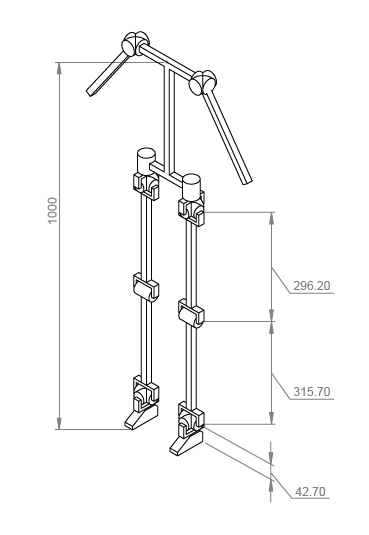
\includegraphics[width=0.45\textwidth]{chapter3/images/uthai_structure1.png}
    \caption{ภาพแสดงแสดงโครงสร้างของหุ่นยนต์ UTHAI}
    \label{fig:uthai_structure1}
\end{figure}

เมื่อเราได้แบบจำลองของหุ่นยนต์ฮิวมานอยด์ออกมาแล้ว ลำดับต่อไปคือการกำหนดตำแหน่งการติดตั้งเซนเซอร์และตัวขับเคลื่อนต่างๆเข้าไป
โดยมี Ground contact sensor ติดตั้งที่ใต้ฝ่าเท้าของหุ่นยนต์, IMU sensor ติดตั้งไว้ให้ใกล้กับจุด COM ของหุ่นยนต์ และ Dynamixel servo
ติดตั้งไว้ที่ข้อต่อในแต่ละข้อต่อ
\clearpage

\begin{figure}[ht]
    \centering
    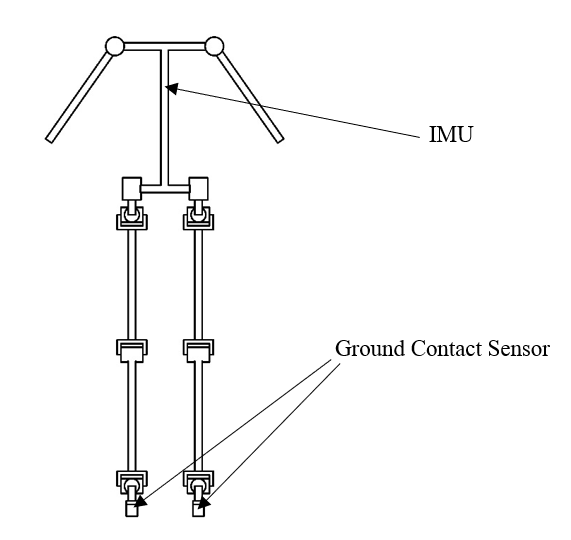
\includegraphics[width=0.5\textwidth]{chapter3/images/uthai_sensor.PNG}
    \caption{ภาพแสดงการติดตั้งเซนเซอร์ในจุดต่างๆ}
    \label{fig:uthai_structure2}
\end{figure}

ส่วนโครงสร้างหุ่นยนต์ฮิวมานอยด์ UTHAI ทางผู้วิจัยเลือกใช้วัสดุหลักเป็น PLA ที่ขึ้นรูปด้วยวิธีการขึ้นรูปสามมิติ
และมีวัสดุเสริมบางชิ้นส่วนจากอลูมิเนียม เนื่องจากจะทำให้โครงสร้างมีน้ำหนักเบา สามารถปรับปรุงแก้ไขง่าย และมีราคาที่สมเหตุสมผล
\begin{table}[ht]
	\centering
	\begin{tabular}{| l | l | l |}
		\hline
		Material & Longitudinal Tensile Strength ($ksi$) & Density ($g/cm^3$) \\
        \hline
        Carbon Fiber & 300 & 1.55 \\
        Steel & 100	& 7.7 \\
        Titanium & 120 & 4.34 \\
        Aluminum & 35 & 2.7 \\
        PLA 3D printing (50 \% infill) & 3.5 & 1.26 \\
        PLA 3D printing (100 \% infill) & 5.5 & 1.26 \\
	    \hline
	\end{tabular}
	\caption{ตารางแสดงสมบัติทางกลของวัสดุต่าง ๆ}
	\label{tab:material_properties}
\end{table}

\clearpage
\subsection{จัดทำชิ้นส่วนโครงสร้างและประกอบ}
ในกาารจัดทำชิ้นส่วนโครงสร้างนั้นทางผู้จัดทำได้คำนึงถึงความแข็งแรงเป็นหลักซึ่งมีความสำคัญมาก
ในการเคลื่อนที่ของหุ่นยนต์ และยังคงต้องมีน้ำหนักที่เบาอีกด้วย ดังนั้นจึงได้ใช้การขึ้นรูปชิ้นงานด้วยเทคนิค
การพิมพ์ 3 มิติ โดยจะใช้วัสดุหลักเป็นพลาสติก PLA ซึ่งมีความแข็งมากกว่าและขึ้นรูปง่ายกว่าพลาสติกชนิด ABS
เพื่อให้ตอบโจทย์กับหุ่นยนต์แพลตฟอร์มเพื่อพัฒนาต่อยอดในอนาคต ซึ่งผู้ใช้ทุกคนสามารถพิมพ์ขึ้นมาได้ด้วยตนเอง
\footnote{ Printing Guide [https://filaments.ca/pages/temperature-guide]}
\footnote{ PLA vs ABS [https://www.3dhubs.com/knowledge-base/pla-vs-abs-whats-difference]}

\begin{table}[ht]
	\centering
	\begin{tabular}{| l | l | l |}
		\hline
		Properties & ABS & PLA \\
        \hline
        Tensile Strength & 27 $MPa$ & 37 $MPa$ \\
        Elongation & 3.5 \- 50\% & 6\% \\
        Flexural Modulus & 2.1 \- 7.6 $GPa$ & 4 $GPa$ \\
        Density & 1.0 - 1.4 $g/cm^3$ & 1.3 $g/cm^3$ \\
        Melting Point & 230$°C$ - 240$°C$ & 215$°C$ - 235$°C$ \\ 
        การย่อยสลายทางธรรมชาติ & ไม่ได้ & ได้(ภายใต้เงื่อนไขที่ถูกต้อง) \\
	    \hline
	\end{tabular}
	\caption{ตารางแสดงสมบัติทางกลของวัสดุพลาสติก}
	\label{tab:plastic_material_properties}
\end{table}



\subsection{การเชื่อมต่อหุ่นยนต์ฮิวมานอยด์}
โครงสร้างแพลตฟอร์มหุ่นยนต์อุทัยจะประกอบไปด้วยสองขา เพื่อทำให้เกิดองศาอิสระเป็น 12 องศาอิสระ
(DOFs) ใช้ Dynamixel servos 12 ตัว มอเตอร์ Dynamixel ทั้งหมดเชื่อมต่อกันแบบ daisy chain
ข้างนึงของมอเตอร์ตัวแรกเชื่อมต่อกับแบตเตอร์รี่ 12V และอีกข้างต่อกับ USB2Dynamixel
ทั้งหมดนี้เป็นการเชื่อมต่อ Odroid เข้ากับหุ่นยนต์ ดังรูปที่ %\ref{fig:odroid2dynamixel}

% \begin{figure}[ht]
%     \centering
%     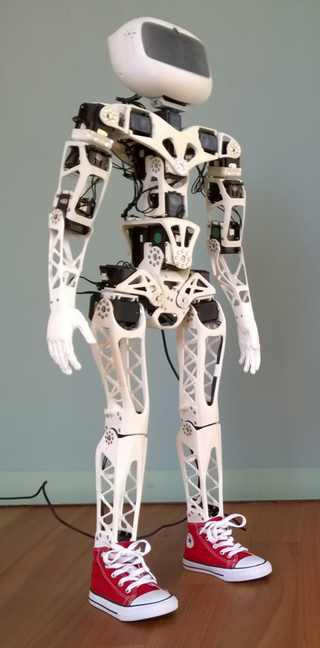
\includegraphics[width=0.3\textwidth]{chapter2/images/PoppyHumanoid1.png}
%     \caption{การเชื่อมต่อระหว่าง Odroid กับ Dynamixel servos}
%     \label{fig:odroid2dynamixel}
% \end{figure}

หุ่นยนต์ฮิวมานอยด์อุทัยใช้เซอร์โวมอเตอร์ 12 ตัว ทำให้เกิดเป็น 12 องศาอิสระ
USB2Dynamixel ใช้เพื่อที่จะสั่งการเซอร์โวมอเตอร์ Dynamixel ผ่าน Odroid
ตำแหน่งของเซอร์โวมอเตอร์ Dynamixel EX-106+ นั้นมาจากเอนโคดเดอร์ที่อยู่ภายใน
เซนเซอร์ Gyro/Accelerometer ติดอยู่กับตัวของหุ่นยนต์ เพื่อช่วยในการทรงตัวของหุ่นยนต์
เซนเซอร์ Accelerometer จะอัพเดตค่าของตัวเองเรื่อยๆ ฟังก์ชั่นส่วนเสริมจะมาจาก ROS
และ Odroid เชื่อมต่อกับคอมพิวเตอร์ภายนอกผ่าน Wi-Fi

\clearpage
\subsection{อุปกรณ์ที่ใช้ในหุ่นยนต์ฮิวมานอยด์อุทัย}

\subsubsection*{Dynamixel servo EX-106+}
Dynamixel EX-106+ เป็นตัวขับเคลื่อนที่นิยมใช้ในปัจจุบัน ซึ่งเป็นเซอร์โวมอเตอร์ที่เหมาะสำหรับทำหุ่นยนต์โดยเฉพาะ
ภายในประกอบไปด้วย มอเตอร์กระแสตรง ชุดเฟืองมอเตอร์ ไดรเวอร์คอนโทรเลอร์ สามารถเชื่อมต่อกันผ่าน BUS RS-485
\footnote{ Robot Actuator [http://support.robotis.com/en/product/actuator/dynamixel/ex\_series/ex-106.htm] }
มีการควบคุมแบบ PID สามารถที่จะอ่านค่าความเร็ว
แรงดันไฟฟ้า กระแสไฟฟ้า อุณหภูมิ ตำแหน่ง และแรงบิดจากมอเตอร์ทุกตัวได้ แต่ละมอเตอร์แต่ละตัวจะมีบอร์ดควบคุมของตัวเอง
เราสามารถที่จะจ่ายไฟให้มอเตอร์และควบคุมผ่าน Serial ได้เลย

การทำงานของตัวขับเคลื่อนนี้สามารถทำได้ 2 รูปแบบคือ\footnote{ EX-106+ Mode [http://www.trossenrobotics.com/dynamixel-ex-106-robot-actuator.aspx] }

\paragraph*{Joint Mode}
สามารถที่จะควบคุม Torque Speed และ position ได้ความละเอียดในการควบคุม 10-bit (0-1023) หมุนได้อยู่ในช่วง 0-250 องศา

\paragraph*{Wheel Mode}
สามารถที่จะควบคุม Torque Speed และ direction ได้ ความละเอียดของความเร็วมอเตอร์เท่ากับ 10bit (0-1023) สามารถหมุนได้ครบ 360 องศาได้

\begin{figure}[ht]
    \centering
    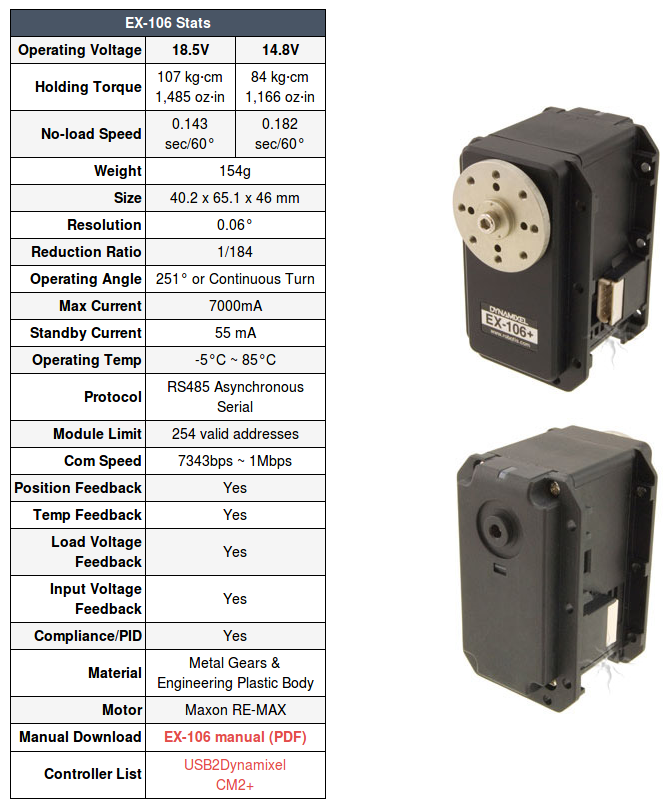
\includegraphics[width=0.75\textwidth]{chapter3/images/dxl_ex106.png}
    \caption{แสดงประสิทธิภาพของมอเตอร์ EX-106+}
    \label{fig:dxl_ex106}
\end{figure}

\clearpage


\subsubsection*{USB2Dynamixel connector}
USB2Dynamixel เป็นอุปกรณ์สำหรับเชื่อมต่อ Odroid กับ Dynamixel โดยจะเชื่อมต่อผ่านพอร์ท USB ของ Odroid ไปยัง Dynamixel motor
ผ่านสายทั้งหมด 4 เส้น เป็นการเชื่อมต่อแบบ RS-485\footnote{USB2Dynamixel [http://support.robotis.com/en/product/auxdevice/interface/usb2dxl\_manual.html]}

\begin{figure}[ht]
    \centering
    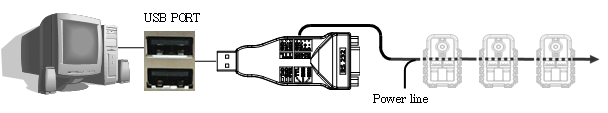
\includegraphics[width=0.75\textwidth]{chapter3/images/dynamixel2pc.png}
    \caption{ภาพแสดงการติดต่อสื่อสารระหว่าง PC กับมอเตอร์ Dynamixel}
    \label{fig:dynamixel2pc}
\end{figure}


ในการต่อใช้งานนั้นผู้ใช้งานจำเป็นต้องเลือกการติดต่อสื่อสารระหว่าง คอมพิวเตอร์กับ มอเตอร์ ซึ่งการติดต่อสื่อสารนั้น
USB2Dynamixel ได้แบ่งการติดต่อสื่อสารออกเป็น 3 ส่วนคือ
\begin{enumerate}
    \item TTL Communication : สำหรับมอเตอร์ Dynamixels ที่ใช้พอร์ทชนิด 3-pin เช่นในตระกูล AX Series เช่น AX-S1 AX-12+ ฯลฯ
    \item  RS485 Communication : สำหรับมอเตอร์ Dynamixels ที่ใช้พอร์ทชนิด 4-pin port เช่นในตระกูล DX Series เช่น RX Series, EX Series ฯลฯ
    \item RS232 Communication : ใช้สำหรับติดต่อสื่อสารกับ controller ผ่านสายเคเบิลเช่น CM-5, CM-510 ฯลฯ
\end{enumerate}

\begin{figure}[ht]
    \centering
    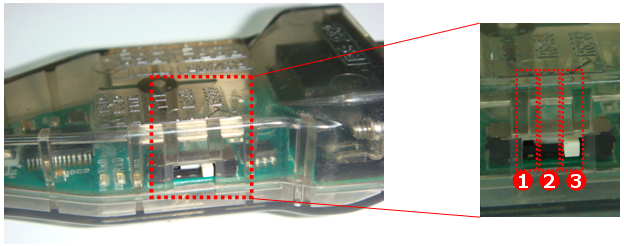
\includegraphics[width=0.75\textwidth]{chapter3/images/useusb2dynamixel.png}
    \caption{ภาพแสดงการเลือกโหมดใช้งานของ USB2Dynamixel}
    \label{fig:useusb2dynamixel}
\end{figure}

\subsubsection*{Inertial Measurement Unit (IMU)}
ในการทำวิจัยครั้งนี้ผู้จัดทำได้เลือกนำเซนเซอร์ MPU-9250 มาใช้ในการอ่านค่ามุมเอียงของหุ่นยนต์เพื่อใช้ในการคุมเสถียรภาพของหุ่นยนต์
โดยเซนเซอร์ตัวนี้สามารถวัดค่าได้ 9 แกนคือ วัดค่าความเร็วเชิงมุม(gyroscope) 3 แกน วัดค่าความเร่งเชิงเส้น(accelerometer) 3 แกน
และวัดค่าสนามแม่เหล็กโลก({magnetometer) 3 แกน ซึ่งเซนเซอร์ตัวนี้จะติดตั้งบริเวณส่วนของลำตัวหุ่นยนต์
เนื่องจากว่าจะเป็นจุดที่สามารถบ่งบอกได้ถึงการเคลื่อนที่และมุมเอียงของหุ่นยนต์ในขณะนั้นได้ดีที่สุด\footnote{ MPU-9250 [http://www.arduiner.com/en/gy-series-axis-accellerometers/6924-gy9255-mpu9255-sensor-module-alternative-mpu9150-mpu9250-3809200640200.html] }
\begin{figure}[ht]
    \centering
    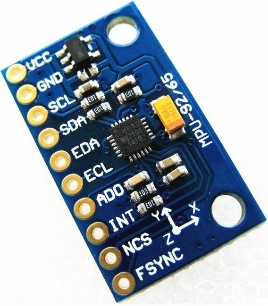
\includegraphics[width=0.2\textwidth]{chapter3/images/mpu9250.jpeg}
    \caption{แสดงเซนเซอร์ IMU MPU9250}
    \label{fig:mpu9250}
\end{figure}

\subsubsection*{Ground contact sensor}
เซนเซอร์ตรวจหน้าสัมผัสที่พื้นเป็นเซนเซอร์ที่ถูกติดตั้งบริเวณฝ่าเท้า เพื่อตรวจสอบการเดินของหุ่นยนต์ฮิวมานอยด์ว่าขณะนี้มีการสัมผัสของฝ่าเท้าของหุ่นยนต์กับพื้นหรือไม่ 
ซึ่งในงานวิจัยนี้ได้ใช้หลักการตัวตรวจจับแรงกดแบบค่าความต้านทานหรือ Force Sensing Resistor (FSR) ที่ใช้เทคโนโลยีฟิล์มโพลีเมอร์แบบหนา (Polymer Thick Film) 
โดยแรงดันไฟฟ้าที่ตกคร่อมตัวตรวจจับจะลดลง เมื่อมีแรงกดมากระทำบนแผ่นตรวจจับ มีโครงสร้างของตัวตรวจจับแสดงในรูปที่\ref{fig:FSRarchitec}
\begin{figure}[ht]
    \centering
    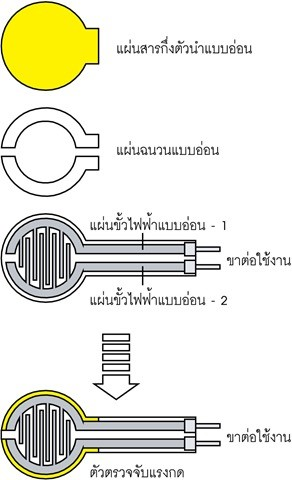
\includegraphics[width=0.35\textwidth]{chapter3/images/FSRarchitec.jpg}
    \caption{ลักษณะโครงสร้างของตัวตรวจจับแรงกด FSR}
    \label{fig:FSRarchitec}
\end{figure}

ประกอบด้วยแผ่นสารกึ่งตัวนำแบบอ่อนที่เป็นตัวกำหนดค่าความต้านทานไฟฟ้าประกบ เข้ากับแผ่นขั้วไฟฟ้าแบบอ่อน โดยมีแผ่นฉนวนแบบอ่อนคั่นกลาง 
ทำให้เกิดค่าความต้านทานไฟฟ้าขึ้นระหว่างขาต่อใช้งาน เมื่อมีการกดลงบนแผ่นขั้วนำไฟฟ้า จะทำให้เกิดการสัมผัสระหว่างสารกึ่งตัวนำกับขั้วไฟฟ้า
ส่งผลให้ค่าความต้านทานไฟฟ้าเกิดการเปลี่ยนแปลง ดังแสดงกระบวนการทำงานในรูปที่\ref{fig:fig:FSRfunction}
\begin{figure}[ht]
    \centering
    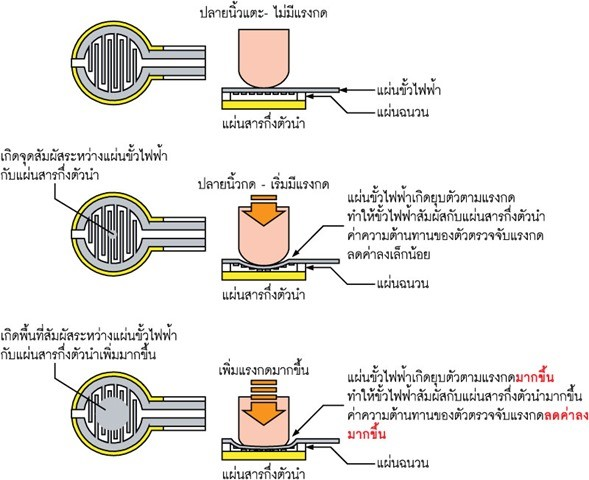
\includegraphics[width=1.0\textwidth]{chapter3/images/FSRfunction.jpg}
    \caption{การทำงานของตัวตรวจจับแรงกด FSR}
    \label{fig:FSRfunction}
\end{figure}


\subsubsection*{Wi-Fi Adapter}
\begin{figure}[ht]
    \centering
    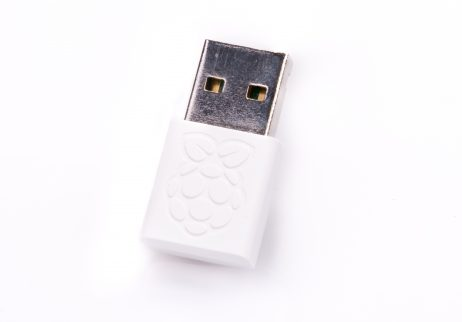
\includegraphics[width=0.3\textwidth]{chapter3/images/rpi_wifi_adaptor.jpg}
    \caption{ตัวรับสัญญาณ wifi ของ RaspberryPi}
    \label{fig:rpi_wifi_adaptor}
\end{figure}

ตัวรับสัญญาณ wifi ชนิดพกพาเพื่อใช้ในการติดต่อสื่อสารระหว่างคอมพิวเตอร์และบอร์ดควบคุม ซึ่งในโครงงานนนี้
จะใช้ส่งข้อมูลที่ต้องการ การประมวลผลบนคอมพิวเตอร์เช่น การวางแผนการเดิน การคำนวนเรื่องพลศาสตร์ของหุ่นยนต์
โดยจะมีตัวกลางในการรับส่งสัญาณผ่านตัวกระจายสัญญาณ(wifi router) 

